\section{The Boltzmann Equation}
At high altitudes or in high speed flows the gas is best described at microscopic level using the velocity distribution function $f(\vec{x},\vec{u},t)$. The distribution function is defined by the property that $f(\vec{x},\vec{u},t)d\vec{x} d\vec{u}$ gives the number of molecules in a volume of size $d\vec{x}$ near point $\vec{x}$ whose velocities are contained in the volume of size $d\vec{u}$ near point $\vec{u}$. In 1872 Boltzmann \cite{boltzmann} introduced an equation which describes the evolution of the velocity distribution function. If there are no external forces such as gravity and if particle density is low enough that one can neglect the effect of particle collisions, then the time evolution of the velocity distribution function is governed by the following transport equation
%
\begin{equation}
\label{no_collision}
\partial_t f(\vec{x},\vec{u},t) + \vec{u} \cdot \nabla_x f(\vec{x},\vec{u},t) = 0.
\end{equation}
%
Note that (\ref{no_collision}) describes a rarefied state of particles where collisions are rare. This can be observed at high altitudes of the atmosphere where the density is very low. However, at lower altitudes the density of the atmosphere is higher and we cannot neglect the effects of the collision of particles. Therefore (\ref{no_collision}) needs to be replaced by (\ref{with_collision}) below where the source term $\Psi$ is the term responsible for the collisions.
%
\begin{equation}
\label{with_collision}
\partial_t f(\vec{x},\vec{u},t) + \vec{u} \cdot \nabla_x f(\vec{x},\vec{u},t) = \Psi(f(\vec{x},\vec{u},t)).
\end{equation}
%
Let us briefly describe the derivation of the Boltzmann collision operator $\Psi$. We will need a few assumptions about the gas. First, we assume that the gas consists of molecules of the same kind. Second, we perform our derivation in a particular case when particles are assumed to be hard spheres that collide with perfect elasticity. Consequently, the molecules transfer only kinetic energy during collisions. Such scenarios are observed in inert gases such as Neon and Argon where there is no interaction potential between gas particles.

We begin by observing the collision of two particles. Let $\vec{c}_1$ and $\vec{c}_2$ be the pre-collision velocities of particles $p_1$ and $p_2$ and let $\vec{c}_1'$ and $\vec{c}_2'$ be the post collision velocities of the same two particles. Because the particles' momentum is conserved during the collision process, the pre- and post-collision particle velocities obey the following relation:
%
\begin{equation}
m_1 \vec{c}_1 + m_2 \vec{c}_2 = m_1 \vec{c}_1' + m_2 \vec{c}_2'.
\end{equation}
%
Furthermore, according to our assumption the interaction of our two particles are perfectly elastic. Therefore the kinetic energy of the system of two particles is preserved
%
\begin{equation}
\frac{1}{2} m_1 ||\vec{c}_1||^2 + \frac{1}{2} m_2 ||\vec{c}_2||^2 = \frac{1}{2} m_1 ||\vec{c}_1'||^2 + \frac{1}{2} m_2 ||\vec{c}_2'||^2.
\end{equation}
%
Due to our first assumption, we can drop $m_1$ and $m_2$ from both equations. Let's define the vectors of pre-collision relative velocity $\vec{g} = \vec{c}_1 - \vec{c}_2$ and post-collision relative velocity $\vec{g}' = \vec{c}_1' - \vec{c}_2'$ of particle $p_1$ with respect to particle $p_2$. Let $\hat{n}$ be the unit vector in the direction of the segment connecting the centers of the colliding spheres. It can be easily verified that in the case of an elastic collision, $\hat{n}$ can be expressed using the vectors of relative velocities as follows.
%
\begin{equation}
\hat{n} = \frac{\vec{g} - \vec{g}'}{||\vec{g} - \vec{g}'||}.
\end{equation}
%
\begin{figure}[h!]
\label{colliding_spheres}
\centering
  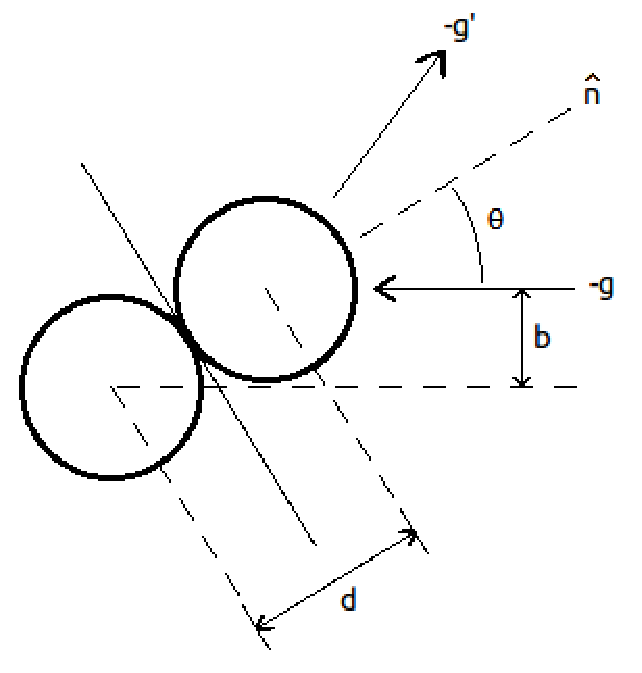
\includegraphics[angle=0,width=80mm]{Boltzmann/colliding_spheres.pdf}
\caption{Collision of two spheres}
\end{figure}
\FloatBarrier
% within the volume $g \, f \, dt \, dc_2 \, db \, d\epsilon$.
An illustration of the collision process can be seen in Figure~(\ref{colliding_spheres}). Consider the coordinate frame with the origin at the center of particle $p_2$ and the x-axis directed parallel to the vector of relative velocity $\vec{g}$. Let particle $p_1$ approach particle $p_2$ in this frame of reference with some offset $b$ at some azimuth angle $\epsilon$. During the time segment $dt$, particle $p_1$ will experience $f_2 g b \, dt \, d\vec{c}_2 \, db \, d\epsilon$ total collisions. We wish to sum over all possible values of the variables $b$, $\epsilon$ and $c$. These variables have constraints that must be determined for collision to happen. The offset $b$ must be between $0$ and the length of the particle diameter $b_*$ and $\epsilon$ can range from $0$ to $2 \pi$. Therefore, the total number of collisions per unit of time over some differential velocity segment $d\vec{c}$ is
%
\begin{equation}
\label{Collide}
\int_{\mathbb{R}^3} \int_0^{2 \pi} \int_0^{b_*} f f_1 g b \, db \, d\epsilon d\vec{c}_2 \, d\vec{c}.
\end{equation}
%
The term (\ref{Collide}) is known as the loss term and it accounts for particles with velocity $\vec{c}$ that will be lost in the result of colliding with other particles. At the same time, new particles with velocity $\vec{c}$ will be created as particles with velocities $\vec{c}'$ and $\vec{c}_1'$ collide at the offset $b$ and azimuth $\epsilon$. Let $f'=f(\vec{x},\vec{c}',t)$ and $f'_1=f(\vec{x},\vec{u}_1',t)$. The total number of particles with velocity $\vec{c}$ that are created during the collision process is given by the following integral known as the gain term
%
\begin{equation}
\label{invCollide}
\int_{\mathbb{R}^3} \int_0^{2 \pi} \int_0^{b_*} f' f_1' g b \, db \, d\epsilon d\vec{c}_1 \, d\vec{c}.
\end{equation}
%
Combining (\ref{Collide}) with (\ref{invCollide}) we arrive at the expression for the Boltzmann integral
%
\begin{equation*}
\label{BoltzmannRHS}
\Psi(f) = \int_{\mathbb{R}^3} \int_0^{2 \pi} \int_0^{b_*} \left( f' f_1' - f f_1 \right) g b \, db \, d\epsilon \, d\vec{c}_1.
\end{equation*}
%
Substituting this into (\ref{with_collision}) we obtain the Boltzmann equation
%
\begin{equation*}
\partial_t f + \vec{u} \cdot \nabla_x f = \int_{\mathbb{R}^3} \int_0^{2 \pi} \int_0^{b_*} \left( f' f_1' - f f_1 \right) \vec{g} b \, db \, d\epsilon \, d\vec{c}_1.
\end{equation*}
%
This is a non-linear integro-differential equation describing the evolution of $f(\vec{x},\vec{u},t)$.
%%%%%%%%%%%%%%%%%%%%%%%%%%%%%%%%%%%%%%%%%%%%%%%%%%%%%%%%%%%%%%%%%%%%%%%%%%%%
%%%%%%%%%%%%%%%%%%%%%%%%%%%%%%%%%%%%%%%%%%%%%%%%%%%%%%%%%%%%%%%%%%%%%%%%%%%%
%%%%%%%%%%%%%%%%%%%%%%%%%%%%%%%%%%%%%%%%%%%%%%%%%%%%%%%%%%%%%%%%%%%%%%%%%%%%
\subsection{The Maxwellian Distribution}
If the system of gas particles are not influenced by any outside intervention, then the distribution of gas particles will approach a state of equilibrium. The equilibrium distribution has the following form
%
\begin{equation}
\label{theDist}
f_0(\vec{u}; a,b,c) = a  \exp{\left(-\frac{||\vec{u} - \vec{c}||^2}{b^2}\right)}
\end{equation}
%
where constants $a$, $b$, and $\vec{c}$ depend on the state of gas and will be defined later. Traditionally, gas at the state of equilibrium is described using five parameters: gas density, temperature and the three components of the gas stream velocity. These parameters can be determined from the velocity distribution function by integration. Specifically, we have 
%
\begin{align*}
%\label{density}
n &= \int_{\mathbb{R}^3} f d\vec{u} \quad &\text{(Number Density)}\\
%\label{momentum}
\bar{u}_i &= \frac{1}{n} \int_{\mathbb{R}^3} u_i f d\vec{u} \quad &\text{(Average Velocity)}\\
&\text{and}\\
%\label{temperature}
T &= \frac{1}{3 n R} \int_{\mathbb{R}^3} ||u - \bar{u}||^2 f d\vec{u} \quad &\text{(Temperature)}.
\end{align*}
%
Where $R$ is the specific gas constant. As a consequence the Maxwellian equilibrium distribution takes the form
%
\begin{equation*}
%\label{Maxwellian}
f_M(\vec{u};n,\vec{\bar{u}},T,R) = \frac{n}{\sqrt{(2 \pi R T)^3}}  \exp{\left(-\frac{||\vec{u} - \vec{\bar{u}}||^2}{2 R T}\right)}
\end{equation*}
%
\begin{figure}[h!]
  \centering
      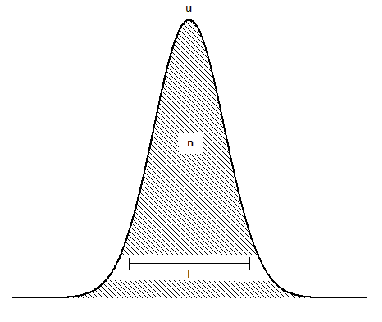
\includegraphics[angle=0,width=70mm]{Boltzmann/Maxwellian.pdf}
  \caption{\label{Max_fig}A Maxwellian distribution defined by the number density, bulk velocity and temperature.}
\end{figure}
\FloatBarrier
%
Figure~(\ref{Max_fig}) illustrates Maxwellian equilibrium distribution. The temperature is a quantity that describes how quickly the gas molecules are moving with respect to each other. The faster the molecules move, the higher the temperature and so the deviation from the mean velocity will be higher. The mean velocity we obtain from the average of the distribution function. The number density is the molecular count of the number of molecules in the gas and this is the area under the curve of the Maxwellian. When the gas has the distribution of the Maxwellian, we say the gas has reached a state of continuum.
%%%%%%%%%%%%%%%%%%%%%%%%%%%%%%%%%%%%%%%%%%%%%%%%%%%%%%%%%%%%%%%%%%%%%%%%%%%%
%%%%%%%%%%%%%%%%%%%%%%%%%%%%%%%%%%%%%%%%%%%%%%%%%%%%%%%%%%%%%%%%%%%%%%%%%%%%
%%%%%%%%%%%%%%%%%%%%%%%%%%%%%%%%%%%%%%%%%%%%%%%%%%%%%%%%%%%%%%%%%%%%%%%%%%%%
%%%%%%%%%%%%%%%%%%%%%%%%%%%%%%%%%%%%%%%%%%%%%%%%%%%%%%%%%%%%%%%%%%%%%%%%%%%%
%%%%%%%%%%%%%%%%%%%%%%%%%%%%%%%%%%%%%%%%%%%%%%%%%%%%%%%%%%%%%%%%%%%%%%%%%%%%
%%%%%%%%%%%%%%%%%%%%%%%%%%%%%%%%%%%%%%%%%%%%%%%%%%%%%%%%%%%%%%%%%%%%%%%%%%%%
%%%%%%%%%%%%%%%%%%%%%%%%%%%%%%%%%%%%%%%%%%%%%%%%%%%%%%%%%%%%%%%%%%%%%%%%%%%%
\section{Model Kinetic Equations}
To evaluate the Boltzmann collision operator we need to calculate a five fold integral. Integral in three dimensions in velocity space and in two dimensions in the collision impact parameter space. Because of the complexity of the collision integral closed form solutions to the Boltzmann equation are extremely difficult to obtain. Such solutions are only known in a few special cases. In general, one can only hope to compute approximate solutions numerically. However, even a numerical solution of the Boltzmann equation is extremely challenging because its straightforward discretization requires $O(n^{11})$ operations. We will look into the deterministic numerical solution of the Boltzmann equation in a later chapter. In this chapter, we are interested in the solutions to simpler approximate models of the Boltzmann equation. These models are the model kinetic equations. In 1954 Bhatnagar, Gross and Krook have proposed the BGK method in their paper \cite{bgk} to approximate the Boltzmann equation by replacing the collision integral with a term that relaxes the solution to the local Maxwellian. The BGK model supports the right hydrodynamic limit but its solution does not does not satisfy the Navier-Stokes equations. The problem is that the BGK model incorrectly predicts the Prandtl number. In particular, the number is always $1$ in the BGK solutions while for monotonic gases like Argon is expected to be about $2/3$. Later Holway \cite{esbgk} has proposed the Ellipsoidal-Statistical BGK or ES-BGK method which, similar to the BGK method, replaces the Boltzmann collision operator with a relaxation equation. The difference is that the target equilibrium distribution function in the ES-BGK model is a Gaussian distribution. The ES-BGK model achieves the correct Prandtl number. Also, it gives closer approximations to the Boltzmann equation at higher densities.
%%%%%%%%%%%%%%%%%%%%%%%%%%%%%%%%%%%%%%%%%%%%%%%%%%%%%%%%%%%%%%%%%%%%%%%%%%%%
%%%%%%%%%%%%%%%%%%%%%%%%%%%%%%%%%%%%%%%%%%%%%%%%%%%%%%%%%%%%%%%%%%%%%%%%%%%%
%%%%%%%%%%%%%%%%%%%%%%%%%%%%%%%%%%%%%%%%%%%%%%%%%%%%%%%%%%%%%%%%%%%%%%%%%%%%
%%%%%%%%%%%%%%%%%%%%%%%%%%%%%%%%%%%%%%%%%%%%%%%%%%%%%%%%%%%%%%%%%%%%%%%%%%%%
\subsection{The BGK Model}
In this section we will derive the kinetic BGK model and show that it conserves mass, momentum and energy which are the first three moments of the distribution function through velocity. This property of the BGK system is due to the fact that it relaxes the solution to the local Maxwellian. From Strutchtrup \cite{struchtrup}, we begin by taking the post collision terms and assuming they are near the Maxwellian $f_1' \approx f_{M 1}'$ and $f' \approx f_M'$. As a result, $f_M' f_{M1}' = f_M f_{M1}$ so then the collision integral term of the Boltzmann equation simplifies into
\begin{equation*}
f_m \int_{\mathbb{R}^3} \int_0^{2 \pi} \int_0^{b_*} f_{M1} g b db \, d\epsilon \, du' - f \int_{\mathbb{R}^3} \int_0^{2 \pi} \int_0^{b_*} f_1 g b db \, d\epsilon \, du'
\end{equation*}
%
We can assume that
\begin{equation*}
\label{difficultnu}
\nu = \int_{\mathbb{R}^3} \int_0^{2 \pi} \int_0^{b_*} f_{M1} g b db \, d\epsilon \, du' \approx \int_{\mathbb{R}^3} \int_0^{2 \pi} \int_0^{b_*} f_1 g b db \, d\epsilon \, du'
\end{equation*}
%
Where we arrive at the BGK collision operator
\begin{equation}
\label{BGK}
\Psi_{BGK}(f) = \nu_{BGK} \left(f_M - f \right).
\end{equation}
%
The BGK equation takes the form
%
\begin{equation}
\label{BGKeq}
\partial_t f + \vec{u} \cdot \nabla_x f = \nu_{BGK} \left(f_M - f \right).
\end{equation}
%
Because it is impractical to compute the collision frequency using formula (\ref{difficultnu}), it usually replaced by the mean the mean collision frequency as a ratio of the pressure and the dynamic viscosity
\begin{equation}
\label{collision}
\nu_{BGK} = \frac{P}{\mu}.
\end{equation}
%
Where the dynamic viscosity is computed from
\begin{equation}
\mu = \mu_0 (T/T_{ref})^{\alpha_{gas}}
\end{equation}
%
and the pressure is obtained from $P = n k T$ where $n$ is the number density and $k$ is the Boltzmann constant. Let us compute the first three moments of ($\ref{BGK}$), obtained by a multiplication of the BGK operator $\Psi$ by the functions $\{ 1, u_i, ||\vec{u} - \vec{\bar{u}}||^2 \}$:
%
\begin{itemize}
%%%%%%%%%%%%%%%%%%%%%%%%%%%%%%%%%%%%%%%%%%%%%%%%%%%%%%%%%%%%%%%%%%%%%%%%%%%%%%%%%%%%
\item Case \{ $1$ \}
%
\begin{align*}
\int_{\mathbb{R}^3} \Psi_{BGK} (f) d\vec{u} &= \int_{\mathbb{R}^3} \nu (f_M - f) d\vec{u}\\
&= \nu \left(\int_{\mathbb{R}^3} \frac{n}{\sqrt{(2 \pi R T)^3}} e^{-\frac{||\vec{u} - \vec{\bar{u}}||^2}{2 R T}} d\vec{u} - \int_{\mathbb{R}^3} f d\vec{u} \right)\nonumber \\
&= \nu \left( \frac{n}{\sqrt{(2 \pi R T)^3}} \int_{\mathbb{R}^3} e^{-\frac{||\vec{u} - \vec{\bar{u}}||^2}{2 R T}} d\vec{u} - n \right)\nonumber \\
&= \nu (n - n) = 0.
\end{align*}
%%%%%%%%%%%%%%%%%%%%%%%%%%%%%%%%%%%%%%%%%%%%%%%%%%%%%%%%%%%%%%%%%%%%%%%%%%%%%%%%%%%%
\item Case \{ $u_i$ \}
%
\begin{align*}
\int_{\mathbb{R}^3} &u_i \Psi_{BGK} (f) d\vec{u} = \nu \int_{\mathbb{R}^3} u_i (f_M - f) d\vec{u} \nonumber \\
&= \nu \left( \frac{n}{\sqrt{(2 \pi R T)^3}} \int_{\mathbb{R}^3} u_i e^{-\frac{||\vec{u} - \vec{\bar{u}}||^2}{2 R T}} d\vec{u} - \int_{\mathbb{R}} u_i f d\vec{u} \right)\nonumber \\
&= \nu \left( \frac{n}{\sqrt{(2 \pi R T)^3}} \int_{\mathbb{R}^3} u_i e^{-\frac{(u_i - \bar{u}_i)^2}{2 R T}} du_i \prod_{j=1,3 \atop j \ne i} \int_{\mathbb{R}^3} e^{-\frac{(u_j - \bar{u}_j)^2}{2 R T}} du_j - n \bar{u}_j \right) \nonumber
\end{align*}
%
we can shift the domain by $(\bar{u}_1,\bar{u}_2,\bar{u}_3)$ so that the exponential is centered at zero and set $v_k = u_k/(2 R T)$ for $k=1,2,3$ to get
%
\begin{align*}
= \nu \left( \frac{n \sqrt{(2 R T)^3}}{\sqrt{(2 \pi R T)^3}} \int_{\mathbb{R}^3} (\sqrt{2 R T} v_i + \bar{u}_i) e^{-v_i^2} dv_i \prod_{j=1,3 \atop j \ne i} \int_{\mathbb{R}^3} e^{-v_j^2} dv_j - n \bar{u}_j \right).
\end{align*}
%
Notice that $\int v_i  \exp{\left(-v_i^2\right)} d v_i$ is finite over any domain and odd about zero and so its evaluation over $\mathbb{R}$ is zero. Recalling that $\int_{\mathbb{R}}  \exp{\left(-v_j^2\right)} dv_j = \sqrt{\pi}$ we obtain
%
\begin{equation*}
= \nu (n u_i - n u_i) = 0.
\end{equation*}
%%%%%%%%%%%%%%%%%%%%%%%%%%%%%%%%%%%%%%%%%%%%%%%%%%%%%%%%%%%%%%%%%%%%%%%%%%%%%%%%%%%%
\item Case \{ $||\vec{u} - \vec{\bar{u}}||^2$ \}
%
\begin{align*}
&\int_{\mathbb{R}^3} ||\vec{u} - \vec{\bar{u}}||^2 \Psi_{BGK} (f) d\vec{u} = \nu \int_{\mathbb{R}^3} ||\vec{u} - \vec{\bar{u}}||^2 (f_M - f) d\vec{u}\\
&= \nu \left( \frac{n}{\sqrt{(2 \pi R T)^3}} \int_{\mathbb{R}^3} ||\vec{u} - \vec{\bar{u}}||^2 e^{-\frac{||\vec{u} - \vec{\bar{u}}||^2}{2 R T}} d\vec{u} - \int_{\mathbb{R}} ||\vec{u} - \vec{\bar{u}}||^2 f d\vec{u} \right)\nonumber \\
&= \nu \left( \frac{n}{\sqrt{(2 \pi R T)^3}} \sum_{i=1,2,3} \int_{\mathbb{R}^3} (u_i - \bar{u}_i)^2 e^{-\frac{||u_i - \bar{u}_i||^2}{2 R T}} du_i - 3 n R T \right)\nonumber \\
&= \nu \frac{n}{\sqrt{(2 \pi R T)^3}} \sum_{i=1,2,3} \int_{\mathbb{R}} (u_i - \bar{u}_i)^2 e^{-\frac{(u_i - \bar{u}_i)^2}{2 R T}} du_i \prod_{j=1,2,3 \atop j \ne i} \int_{\mathbb{R}} e^{-\frac{(u_j - \bar{u}_j)^2}{2 R T}} du_j\\
& \, - \nu 3 n R T
\end{align*}
%
We shift by $(u_1,u_2,u_3)$ to get
%
\begin{align*}
= \nu \left( \frac{n}{\sqrt{(2 \pi R T)^3}} \sum_{i=1,2,3} \int_{\mathbb{R}} u_i^2 e^{-\frac{u_i^2}{2 R T}} du_i \prod_{j=1,2,3 \atop j \ne i} \int_{\mathbb{R}} e^{-\frac{u_i^2}{2 R T}} du_j  - 3 n R T \right)
\end{align*}
%
By a change of variables by letting $\sqrt{2 R T} v_i = u_i$, we have
%
\begin{align*}
&= \nu \frac{n}{\sqrt{(2 \pi R T)^3}} \sum_{i=1,2,3} 2 R T \sqrt{(2 R T)^3} \int_{\mathbb{R}^3} v_i^2 e^{-v_i^2} dv_i \prod_{j=1,2,3 \atop j \ne i} \int_{\mathbb{R}} e^{-v_i^2} dv_j\\
& \, - \nu 3 n R T\\
&= \nu \left( \frac{2 n R T \pi}{\sqrt{\pi^3}} \sum_{i=1,2,3} \int_{\mathbb{R}^3} v_i^2 e^{-v_i^2} dv_i - 3 n R T \right)\\
\end{align*}
%
We then proceed to integrate by parts by separating the integral components into $v_i$ and $v_i e^{-v_i^2} dv_i$ which yields
%
\begin{align}
&= \nu \left( \frac{2 n R T \pi}{\sqrt{\pi^3}} \sum_{i=1,2,3} \left(-\frac{1}{2} v_i e^{-v_i^2}|_{-\infty}^\infty + \frac{1}{2} \int_{\mathbb{R}} e^{-v_i^2} dv_i \right) - 3 n R T \right)\nonumber \\
&= \nu \left(3 n R T - 3 n R T \right) = 0.
\end{align}
\end{itemize}
%
And so we conclude the first five moments of the BGK equation are conserved:
%
\begin{align*}
\int_{\mathbb{R}^3} \Psi_{BGK} (f) d\vec{u} &= 0 \quad & (\text{Mass})\\
\int_{\mathbb{R}^3} \left( \begin{array}{c} u_1 \\ u_2 \\ u_3 \end{array} \right) \Psi_{BGK} (f) d\vec{u} &= \left( \begin{array}{c} 0 \\ 0 \\ 0 \end{array} \right) \quad & (\text{Momentum}) \\
\text{and}\\
\int_{\mathbb{R}^3} ||\vec{u} - \vec{\bar{u}}||^2 \Psi_{BGK} (f) d\vec{u} &= 0 \quad & (\text{Temperature})\\
\end{align*}
%
%%%%%%%%%%%%%%%%%%%%%%%%%%%%%%%%%%%%%%%%%%%%%%%%%%%%%%%%%%%%%%%%%%%%%%%%%%%%
%%%%%%%%%%%%%%%%%%%%%%%%%%%%%%%%%%%%%%%%%%%%%%%%%%%%%%%%%%%%%%%%%%%%%%%%%%%%
%%%%%%%%%%%%%%%%%%%%%%%%%%%%%%%%%%%%%%%%%%%%%%%%%%%%%%%%%%%%%%%%%%%%%%%%%%%%
%%%%%%%%%%%%%%%%%%%%%%%%%%%%%%%%%%%%%%%%%%%%%%%%%%%%%%%%%%%%%%%%%%%%%%%%%%%%
%%%%%%%%%%%%%%%%%%%%%%%%%%%%%%%%%%%%%%%%%%%%%%%%%%%%%%%%%%%%%%%%%%%%%%%%%%%%
%%%%%%%%%%%%%%%%%%%%%%%%%%%%%%%%%%%%%%%%%%%%%%%%%%%%%%%%%%%%%%%%%%%%%%%%%%%%
%%%%%%%%%%%%%%%%%%%%%%%%%%%%%%%%%%%%%%%%%%%%%%%%%%%%%%%%%%%%%%%%%%%%%%%%%%%%
\subsection{The ES-BGK Model}
Holway [10] proposed a modification to the BGK model, known as the ellipsoidal-statistical BGK model that achieves the correct Prandtl number. According to Andries \cite{andries} the BGK model has been shown to produce satisfactory results and, a first order Chapman-Enskog expansion applied to ($\ref{BGK}$) gives the correct Navier-Stokes viscosity $\mu$ but gives a heat conduction of $\kappa = (5/2)R \mu$ which results in a Prandtl number of
\begin{equation}
\label{Prandtl}
Pr = \frac{5 R \mu }{2 \kappa} = 1.
\end{equation}
%
For monotonic gases like Argon, the desired Prandtl number is near $Pr = 2/3$ and so the BGK approximation will fail to give the correct Navier-Stokes heat conduction. The ES-BGK model corrects the Prandtl number by the use of an adjustment factor $\alpha$:
%
\begin{equation}
Pr = \frac{1}{1 - \alpha}
\end{equation}
%
where $\alpha$ is a parameter in the tensor 
%
\begin{equation}
\mathbb{T} = (1-\alpha)RT I + \alpha \Theta
\end{equation}
%
and
%
\begin{equation}
\label{Theta}
\Theta_{ij} := \frac{1}{n} \int_{\mathbb{R}^{3}} c_i c_j f \, d\vec{u}.
\end{equation}
%
The ES-BGK relaxation term is
%L.H. Holway. Kinetic theory of shock structure using an ellipsoidal distribution function, in: Rarefied Gas Dynamics, vol. I (Proceedings of the Fourth International Symposium, University of Toronto, 1964), Academic Press, New York, 1966, pp. 193–215.%
%
\begin{equation}
\label{Gaussian}
f_{ES} = \frac{n}{\sqrt{\det(2 \pi \bar{\bar{\mathbb{T}}})}}  \exp{\left(-\frac{\vec{c}' \bar{\bar{\mathbb{T}}}^{-1} \vec{c}}{2}\right)}
\end{equation}
%
where $\vec{c} = \vec{u} - \bar{\vec{u}}$ is the pecular velocity. $f_{ES}$ replaces the Maxwellian in (\ref{BGK}). We expect (\ref{Gaussian}) to approach zero for large values of $\vec{u}$. Also form physical considerations we need $\alpha$ to be chosen so that $\mathbb{T}^{-1}$ or $\mathbb{T}$ is positive definite. Zheng \cite{zheng} has shown that if we restrict $\alpha \in [-\frac{1}{2},1)$, then we preserve the positive definite behavior of $\mathbb{T}$.

The collision frequency for the ES-BGK model is
%
\begin{equation}
\nu_{ES} = \frac{P}{(1 - \alpha) \mu}
\end{equation}
%
and the ES-BGK collision operator takes the form of
%
\begin{equation}
\label{ESBGK}
\Psi_{ES}(f) = \nu_{ES} \left(f_{ES} - f \right)
\end{equation}
%
giving us the ES-BGK equation
%
\begin{equation}
\label{ESBGKeq}
\partial_t f + \vec{u} \cdot \nabla_x f = \nu_{ES} \left(f_{ES} - f \right).
\end{equation}
%
Notice that when $\alpha = 0$ we obtain the original BGK model back suggesting that the ES-BGK model generalizes the BGK model.
%Maximum entropy derivation Junk, M.: Maximum entropy for reduced moment problems. M3AS 10, 1121–1149 (2000)
%%%%%%%%%%%%%%%%%%%%%%%%%%%%%%%%%%%%%%%%%%%%%%%%%%%%%%%%%%%%%%%%%%%%%%%%%%%%%%%%%%%%%%%%%%%
%%%%%%%%%%%%%%%%%%%%%%%%%%%%%%%%%%%%%%%%%%%%%%%%%%%%%%%%%%%%%%%%%%%%%%%%%%%%%%%%%%%%%%%%%%%
%%%%%%%%%%%%%%%%%%%%%%%%%%%%%%%%%%%%%%%%%%%%%%%%%%%%%%%%%%%%%%%%%%%%%%%%%%%%%%%%%%%%%%%%%%%
%%%%%%%%%%%%%%%%%%%%%%%%%%%%%%%%%%%%%%%%%%%%%%%%%%%%%%%%%%%%%%%%%%%%%%%%%%%%%%%%%%%%%%%%%%%
\section{One Dimensional Reduction}
It is in our interest in the rest of this chapter to compute the solution to the model equations constrained to one dimension. We can assume that the solution is not changing in two of the three spatial dimensions that we will denoted as $y$ and $z$. In a physical sense, the gas is held between two infinitely long parallel plates where the mass flux along the planar directions is zero. Reducing our problem to one dimension and using the approximate kinetic models will reduce the computational effort because the integration is done in only one dimension. With this assumption, our objective here is to reduce the three dimensional kinetic model to two separate hyperbolic PDEs of similar form that will be tied together by the calculation of the macro parameters. To accomplish this, we start with introducing the reduced distribution functions $h(x,u_1,t)$ and $g(x,u_1,t)$ by integrating the distribution function $f(\vec{x},\vec{u},t)$ through velocity in the $u_2$ and $u_3$ directions and integrating the product of $f$ and the velocity $u_2$ (in $y$ direction) through $u_2$ and $u_3$ directions of velocity
%
\begin{equation}
\label{f1}
h(x,u_1,t) = \int_{\mathbb{R}^2} f du_2 du_3
\end{equation}
%
and
%
\begin{equation}
\label{f2}
g(x,u_1,t) = \int_{\mathbb{R}^2} u_2^2 f du_2 du_3
\end{equation}
%
which, as we will soon see, will be the catalyst in the reduction process.
%%%%%%%%%%%%%%%%%%%%%%%%%%%%%%%%%%%%%%%%%%%%%%%%%%%%%%%%%%%%%%%%%%%%%%%%%%%%%%%%%%%%%%%%%%%%%%%%%%%%%%%%%%%%%%%%%%%%%%%%%
\subsection{Reduction of the Macro Parameters}
In this section, we will reduce the macro parameters to one dimension. The density can be written as
%
\begin{align*}
n &= \int_{\mathbb{R}^3} f d\vec{u}\\
&= \int_{\mathbb{R}} \left( \int_{\mathbb{R}^2} f du_2 du_3 \right) du_1\\
&= \int_{\mathbb{R}} h du_1.
\end{align*}
%
Next we will reduce the bulk velocity. For the $i^{th}$ component of the bulk velocity we obtain
%
\begin{align*}
\bar{u}_i &= \frac{1}{n} \int_{\mathbb{R}^3} u_i f d\vec{u}\\
&= \frac{1}{n} \int_{\mathbb{R}} \left( \int_{\mathbb{R}^2} u_i f du_2 du_3 \right) du_1
\end{align*}
%
but because there is no mass exchange expected in the $y$ and $z$ directions we obtain
%
\begin{equation*}
\bar{u}_i = \frac{1}{n} \left \{ \begin{array}{cc} \int_{\mathbb{R}} u_1 h du_1 & i=1\\ 0 & i = 2,3 \end{array} \right. .
\end{equation*}
%
The temperature
%
\begin{align*}
T &= \frac{1}{3 n R} \int_{\mathbb{R}^3} ||u - \bar{u}||^2 f d\vec{u}\\
&= \frac{1}{3 n R} \int_{\mathbb{R}^3} \left( ||\vec{u}||^2 - 2 \vec{u} \cdot \vec{\bar{u}} + ||\vec{\bar{u}}||^2 \right) f d\vec{u}\\
\end{align*}
%
because the bulk velocity is only in the $x$ direction, we have that $\bar{u}_2 = 0 = \bar{u}_3$ and so
%
\begin{align*}
&= \frac{1}{3 n R} \int_{\mathbb{R}^3} \left( (u_1^2 + u_2^2 + u_3^2) - 2 u_1 \bar{u}_1 + \bar{u}_1^2 \right) f d\vec{u}\\
&= \frac{1}{3 n R} \int_{\mathbb{R}^3} \left( (u_1 - \bar{u_1})^2 + (u_2^2 + u_3^2)\right) f d\vec{u}\\
&= \frac{1}{3 n R} \int_{\mathbb{R}} \left( (u_1 - \bar{u_1})^2 \right) f du_1\\
& \, + \frac{1}{3 n R} \int_{\mathbb{R}^2} \left( (u_2^2 + u_3^2)\right) f du_2 du_3
\end{align*}
%
based on our symmetry assumption that nothing changes in the $y$ and $z$ directions
%
\begin{equation*}
\int_{\mathbb{R}^3} u_2^2 f du_2 du_3 = \int_{\mathbb{R}^3} u_3^2 f du_2 du_3
\end{equation*}
%
we obtain
%
\begin{equation*}
T = \frac{1}{3 n R} \int_{\mathbb{R}} \left( (u - \bar{u})^2 h + 2 g \right) du_1.
\end{equation*}
%%%%%%%%%%%%%%%%%%%%%%%%%%%%%%%%%%%%%%%%%%%%%%%%%%%%%%%%%%%%%%%%%%%%%%%%%%%%%%%%%%%%%%%%%%%%%%%
%%%%%%%%%%%%%%%%%%%%%%%%%%%%%%%%%%%%%%%%%%%%%%%%%%%%%%%%%%%%%%%%%%%%%%%%%%%%%%%%%%%%%%%%%%%%%%%
%%%%%%%%%%%%%%%%%%%%%%%%%%%%%%%%%%%%%%%%%%%%%%%%%%%%%%%%%%%%%%%%%%%%%%%%%%%%%%%%%%%%%%%%%%%%%%%
%%%%%%%%%%%%%%%%%%%%%%%%%%%%%%%%%%%%%%%%%%%%%%%%%%%%%%%%%%%%%%%%%%%%%%%%%%%%%%%%%%%%%%%%%%%%%%%
\subsection{Reduction of the Kinetic Model}
We begin now to reduce the equation
%
\begin{equation}
\label{kineticModel}
\partial_t f + \vec{u} \cdot \nabla_x f = \nu \left( f_0 - f \right).
\end{equation}
%
to one dimension. Since it is our assumption that the gas is homogeneous in the $y$ and $z$ directions, there is no change and so we expect $\vec{u} \cdot \nabla_x = u \partial_x$. As a result (\ref{kineticModel}) reduces to
%
\begin{equation}
\label{reduction1}
\partial_t f + u \partial_x f = \nu \left( f_0 - f \right).
\end{equation}
%
Now $f$ is still a function of $\vec{x}$ and $\vec{u}$. To reduce the equation to one dimension. The first step is to integrate (\ref{reduction1}) in the $u_2$ and $u_3$ directions and to obtain an equation with $h$. In the second step we multiply (\ref{reduction1}) by $u_2^2$ then integrate in the $u_2$ and $u_3$ directions to get an evolution equation with $g$.
%
\begin{equation}
\label{eq659}
\int_{\mathbb{R}^2} \partial_t f du_2 du_3 + \int_{\mathbb{R}^2} u_1 \partial_x f du_2 du_3 = \int_{\mathbb{R}^2} \nu \left( f_0 - f \right) du_2 du_3
\end{equation}
%
We can immediately see that by substituting (\ref{f1}) into (\ref{eq659}) the equation reduces to
%
\begin{equation*}
\partial_t h + u_1 \, \partial_x h = \int_{\mathbb{R}^2} \nu \left( f_0 - f \right) du_2 du_3.
\end{equation*}
%
Moreover, because of the linearity of the integral we obtain the following form for the right hand side of the equation
%
\begin{equation}
\label{f1Part}
\int_{\mathbb{R}^2} \nu \left( f_0 - f \right) \, du_2 \, du_3 = \nu \left( \int_{\mathbb{R}^2} f_0 \, du_2 \, du_3 - h \right).
\end{equation}
%
To complete the second step we multiply (\ref{reduction1}) by $u_2^2$
%
\begin{equation*}
u_2^2 \, \partial_t f + u_2^2 \, u_1 \, \partial_x f = u_2^2 \, \nu \, \left( f_0 - f \right).
\end{equation*}
%
and integrate through $u_2$ and $u_3$.
%
\begin{equation*}
\int_{\mathbb{R}^2} u_2^2 \partial_t f du_2 du_3 + \int_{\mathbb{R}^2} u_2^2 u_1 \partial_x f du_2 du_3 = \int_{\mathbb{R}^2} u_2^2 \nu \left( f_0 - f \right) du_2 du_3
\end{equation*}
%
\begin{equation*}
\partial_t \int_{\mathbb{R}^2} u_2^2 f du_2 du_3 + u_1 \partial_x \int_{\mathbb{R}^2} u_2^2 f du_2 du_3 = \nu \left( \int_{\mathbb{R}^2} u_2^2 f_0 du_2 du_3 - \int_{\mathbb{R}^2} u_2^2 f du_2 du_3 \right)
\end{equation*}
%
\begin{equation}
\label{f2Party}
\partial_t g + u_1 \partial_x g = \nu \left( \int_{\mathbb{R}^2} u_2^2 f_0 du_2 du_3 - g \right)
\end{equation}
%
which is our second equation. From here, all that is left is to state the formulas for evaluating the equilibrium distributions in BGK and ES-BGK models in terms of $h$ and $g$. Since $f_0$ is a function of $\vec{u}$, careful consideration is required. This step will depend on the kinetic model we are using therefore we consider the integrals for the BGK and ESBGK models separately below.
%%%%%%%%%%%%%%%%%%%%%%%%%%%%%%%%%%%%%%%%%%%%%%%%%%%%%%%%%%%%%%%%%%%%%%%%%%%%%%%%%%%%%%%%%%%%
%%%%%%%%%%%%%%%%%%%%%%%%%%%%%%%%%%%%%%%%%%%%%%%%%%%%%%%%%%%%%%%%%%%%%%%%%%%%%%%%%%%%%%%%%%%%
%%%%%%%%%%%%%%%%%%%%%%%%%%%%%%%%%%%%%%%%%%%%%%%%%%%%%%%%%%%%%%%%%%%%%%%%%%%%%%%%%%%%%%%%%%%%
%%%%%%%%%%%%%%%%%%%%%%%%%%%%%%%%%%%%%%%%%%%%%%%%%%%%%%%%%%%%%%%%%%%%%%%%%%%%%%%%%%%%%%%%%%%%
%%%%%%%%%%%%%%%%%%%%%%%%%%%%%%%%%%%%%%%%%%%%%%%%%%%%%%%%%%%%%%%%%%%%%%%%%%%%%%%%%%%%%%%%%%%%
\subsection{Reduction of the Maxwellian Distribution}
In the BGK model, we have a Maxwellian distribution $f_0 = f_{BGK} = f_M$ and so we can explicitly evaluate the integral of the Maxwellian through $u_2$ and $u_3$
%
\begin{align}
\label{480}
\int_{\mathbb{R}^2} f_0 du_2 du_3 &= \int_{\mathbb{R}^2} \frac{n}{\sqrt{(2 \pi RT)^3}}  \exp{\left(-\frac{||\vec{u} - \vec{\bar{u}}||^2}{2 RT}\right)} du_2 du_3\\
\end{align}
%
and $\vec{\bar{u}} = (\bar{u}_1,0,0)$ then
%
\begin{align*}
&= \frac{n}{\sqrt{(2 \pi RT)^3}} \int_{\mathbb{R}^2}  \exp{\left(-\frac{||u_1 - \bar{u}_1||^2 + u_2^2 + u_3^2}{2 RT}\right)} du_2 du_3\\
&= \frac{n}{\sqrt{(2 \pi RT)^3}}  \exp{\left(-\frac{(u - \bar{u})^2}{2 RT}\right)} \int_{\mathbb{R}^2}  \exp{\left(-\frac{(u_2^2 + u_3^2)}{2 RT}\right)} du_2 du_3.\\
\end{align*}
%
Let $r^2 = u_2^2 + u_3^2$, $r \cos(\theta) = u_2$ and $r \sin(\theta) = u_3$ then
%
\begin{align*}
\int_{\mathbb{R}^2}  \exp{\left(-\frac{(u_2^2 + u_3^2)}{2 RT}\right)} du_2 du_3 &= \int_0^\infty \int_0^{2 \pi}  \exp{\left(-\frac{(r^2)}{2 RT}\right)} r d\theta dr\\
&= 2 \pi RT.
\end{align*}
%
then (\ref{480}) becomes
%
\begin{equation*}
\int_{\mathbb{R}^2} f_0 du_2 du_3 = \frac{n}{\sqrt{2 \pi RT}}  \exp{\left(-\frac{(u - \bar{u})^2}{2 RT}\right)}.
\end{equation*}
%
Now through a similar process, we will evaluate the product of the distribution function with $u_2^2$.
%
\begin{align*}
\int_{\mathbb{R}^2}& u_2^2 f_0 du_2 du_3 = \int_{\mathbb{R}^2} u_2^2 \frac{n}{\sqrt{(2 \pi RT)^3}}  \exp{\left(-\frac{(u - \bar{u})^2}{2 RT}\right)} du_2 du_3\\
&= \frac{n}{\sqrt{(2 \pi RT)^3}} \int_{\mathbb{R}^2} u_2^2  \exp{\left(-\frac{(u - \bar{u})^2}{2 RT} \right)} du_2 du_3\\
&= \frac{n}{\sqrt{(2 \pi RT)^3}}  \exp{\left(-\frac{(u - \bar{u})^2}{2 RT}\right)} \int_{\mathbb{R}^2} u_2^2  \exp{\left(-\frac{(v^2 + w^2)}{2 RT}\right)} du_2 du_3\\
&= \frac{n}{\sqrt{(2 \pi RT)^3}}  \exp{\left(-\frac{(u - \bar{u})^2}{2 RT}\right)} \int_{\mathbb{R}} u_2^2  \exp{\left(-\frac{u_2^2}{2 RT}\right)} du_2 \int_{\mathbb{R}}  \exp{\left(-\frac{u_3^2}{2 RT}\right)} du_3\\
\end{align*}
%
By adjusting the integral
%
\begin{equation}
\int_{\mathbb{R}} u_2^2  \exp{\left(-\frac{u_2^2}{2 RT}\right)} du_2 = (2 R T)^{3/2} \int_{\mathbb{R}} u_2^2  \exp{\left(-u_2^2\right)} du_2
\end{equation}
%
and evaluating by parts by letting $v = u_2$ and $d w = u_2  \exp{\left(-u_2^2\right)} \, du_2$ we obtain
%
\begin{equation}
= 2 (2 R T)^{3/2} \left(-\frac{1}{2} u_2  \exp{\left(-u_2^2\right)}|_{-\infty}^\infty + \frac{1}{2} \int_{\mathbb{R}}  \exp{\left(-u_2^2\right)} \, du_2 \right) = (R T)^{3/2} \sqrt{2 \pi}.
\end{equation}
%
Then we obtain
%
\begin{align*}
\int_{\mathbb{R}^2} u_2^2 f_0 du_2 du_3 &= \frac{n}{\sqrt{(2 \pi RT)^3}}  \exp{\left(-\frac{(u - \bar{u})^2}{2 RT}\right)} \left((R T)^{3/2} \sqrt{2 \pi} \right) \left( \sqrt{2 \pi R T} \right) \\
&= n \sqrt{\frac{R T}{2 \pi}}  \exp{\left(-\frac{(u - \bar{u})^2}{2 RT}\right)}
\end{align*}
%
which is the reduced Maxwellian distribution function in one dimension. The BGK equations in one dimension take the form:
%
\begin{equation*}
\partial_t h + u_1 \partial_x h = \nu_{BGK} \left(\frac{n}{\sqrt{2 \pi RT}}  \exp{\left(-\frac{(u_1 - \bar{u}_1)^2}{2 RT}\right)} - h \right)
\end{equation*}
%
\begin{equation*}
\partial_t g + u_1 \partial_x g = \nu_{BGK} \left( n \sqrt{\frac{R T}{2 \pi}}  \exp{\left(-\frac{(u - \bar{u})^2}{2 RT}\right)} - g \right)
\end{equation*}
%%%%%%%%%%%%%%%%%%%%%%%%%%%%%%%%%%%%%%%%%%%%%%%%%%%%%%%%%%%%%%%%%%%%%%%%%%%%%%%%%%%%%%%%%%%%
%%%%%%%%%%%%%%%%%%%%%%%%%%%%%%%%%%%%%%%%%%%%%%%%%%%%%%%%%%%%%%%%%%%%%%%%%%%%%%%%%%%%%%%%%%%%
%%%%%%%%%%%%%%%%%%%%%%%%%%%%%%%%%%%%%%%%%%%%%%%%%%%%%%%%%%%%%%%%%%%%%%%%%%%%%%%%%%%%%%%%%%%%
%%%%%%%%%%%%%%%%%%%%%%%%%%%%%%%%%%%%%%%%%%%%%%%%%%%%%%%%%%%%%%%%%%%%%%%%%%%%%%%%%%%%%%%%%%%%
%%%%%%%%%%%%%%%%%%%%%%%%%%%%%%%%%%%%%%%%%%%%%%%%%%%%%%%%%%%%%%%%%%%%%%%%%%%%%%%%%%%%%%%%%%%%
\subsection{Reduction of the Gaussian Distribution Function for ES-BGK}
For the ES-BGK model, recall that the Maxwellian distribution is replaced with a general Gaussian distribution:
%
\begin{equation}
\label{fES}
f_0 = f_{ES} = \frac{n}{\sqrt{\det{\left(2 \pi \mathbb{T}\right)}}} \ \exp{\left(-\frac{c' \mathbb{T}^{-1} c}{2} \right)}
\end{equation}
%
as defined by (\ref{Gaussian}) where $\mathbb{T} = (1 - \alpha) RT \mathbb{I} + \alpha \Theta$ and
%
\begin{equation}
\label{Theta_component}
\Theta_{ij} := \frac{1}{n} \int_{\mathbb{R}^{3}} c_i c_j f du
\end{equation}
%
is from (\ref{Theta}). Expanding $\Theta_{i,j}$:
%
\begin{align*}
\Theta_{i,j} &= \frac{1}{n} \int_{\mathbb{R}} c_i c_j f d\vec{u} = \frac{1}{n} \int_{\mathbb{R}} (u_i - \bar{u}_i)(u_j - \bar{u}_j) f d\vec{u}\\
&= \frac{1}{n} \int_{\mathbb{R}} \left( u_i u_j f - u_i \bar{u}_j f - \bar{u}_i u_j f + \bar{u}_i \bar{u}_j f \right) d\vec{u}.
\end{align*}
%
From our assumption that the bulk of the velocity only changes in the $x$ direction we obtain
%
\begin{equation*}
\int_{\mathbb{R}} u_i f d\vec{u} = \bar{u}_i = \left \{ \begin{array}{cc} 0, & i \neq 1\\ \bar{u}_1, & i = 1 \end{array} \right.
\end{equation*}
%
so then the off diagonal components of (\ref{Theta_component}) are zero and for the diagonal components we obtain
%
\begin{equation*}
\Theta_{i,i} = \left \{ \begin{array}{cc} \int_{\mathbb{R}} (u_1 - \bar{u}_1)^2 f_1 du_1, & i = 1\\ \int_{\mathbb{R}} f_2 du_1, & i = 2,3 \end{array} \right..
\end{equation*}
%
One can see that we have $tr(\Theta) = 3 n R T$. Because the off diagonals are zero, $\det(2 \pi \mathbb{T}) = (2 \pi)^3 \prod_{i=1}^3 
\mathbb{T}_{i,i}$ and 
%
\begin{equation*}
\mathbb{T}_{i,j}^{-1} = \left \{ \begin{array}{cc} \frac{1}{\mathbb{T}_{i,i}}, & i=j\\ 0, & i \neq j \end{array} \right. .
\end{equation*}
%
In the numerator of the exponent of (\ref{fES}) we obtain
%
\begin{equation*}
c' \mathbb{T}^{-1} c = (u_1 - \bar{u}_1)^2 \mathbb{T}_1^{-1} + (u_2^2 + u_3^2) \mathbb{T}_2^{-1}.
\end{equation*}
%
Finally (\ref{fES}) becomes
%
\begin{equation}
\label{1D_ES}
f_{ES} = \frac{n}{\sqrt{(2 \pi)^3 \mathbb{T}_1 \mathbb{T}_2^2}} \ \exp{\left(-\frac{1}{2} \left( (u_1 - \bar{u}_1)^2 \mathbb{T}_1^{-1} + (u_2^2 + u_3^2) \mathbb{T}_2^{-1} \right) \right)}.
\end{equation}
%
Evaluating the integral of (\ref{1D_ES}) through $u_2$ and $u_3$
%
\begin{align*}
&\int_{\mathbb{R}^2} f_{ES} d u_2 d u_3 =\\
&= \int_{\mathbb{R}^2} \frac{n}{\sqrt{(2 \pi)^3 \mathbb{T}_1 \mathbb{T}_2^2}} \ \exp{\left(-\frac{1}{2} \left( (u_1 - \bar{u}_1)^2 \mathbb{T}_1^{-1} + (u_2^2 + u_3^2) \mathbb{T}_2^{-1} \right) \right)} du_2 du_3\\
&= \frac{n}{\sqrt{(2 \pi)^3 \mathbb{T}_1 \mathbb{T}_2^2}} \ \exp{\left(-\frac{1}{2} \left( (u_1 - \bar{u}_1)^2 \mathbb{T}_1^{-1} \right) \right)} \int_{\mathbb{R}^2} \ \exp{\left(-\frac{1}{2} \left( (u_2^2 + u_3^2) \mathbb{T}_2^{-1} \right) \right)} du_2 du_3\\
&= \frac{n}{\sqrt{2 \pi \mathbb{T}_1}} \ \exp{\left(-\frac{1}{2} \left( (u_1 - \bar{u}_1)^2 \mathbb{T}_1^{-1} \right) \right)}.
\end{align*}
%
To obtain the second evolution equation, we will need to also consider the integral of the product of $u_2^2$ and (\ref{1D_ES}) through all of $u_2$ and $u_3$
%
\begin{align*}
&\int_{\mathbb{R}^2} u_2^2 f_{ES} d u_2 d u_3 =\\
&= \frac{n}{\sqrt{(2 \pi)^3 \mathbb{T}_1 \mathbb{T}_2^2}} \ \exp{\left(-\frac{1}{2} \left( (u_1 - \bar{u}_1)^2 \mathbb{T}_1^{-1} \right) \right)} \int_{\mathbb{R}^2} u_2^2 \ \exp{\left(-\frac{1}{2} \left( (u_2^2 + u_3^2) \mathbb{T}_2^{-1} \right) \right)} du_2 du_3\\
&= \frac{n \mathbb{T}_2}{\sqrt{(2 \pi)^3 \mathbb{T}_1}} \ \exp{\left(-\frac{1}{2} \left( (u_1 - \bar{u}_1)^2 \mathbb{T}_1^{-1} \right) \right)}
\end{align*}
%
and so we arrive at the two one dimensional equations of the ES-BGK model:
%
\begin{equation*}
\partial_t h + u_1 \partial_x h = \nu_{ES} \left(\frac{n}{\sqrt{2 \pi \mathbb{T}_1}} \ \exp{\left(-\frac{1}{2} \left( (u_1 - \bar{u}_1)^2 \mathbb{T}_1^{-1} \right) \right)} - h\right)
\end{equation*}
%
\begin{equation*}
\partial_t g + u_1 \partial_x g = \nu_{ES} \left( \frac{n \mathbb{T}_2}{\sqrt{(2 \pi)^3 \mathbb{T}_1}} \ \exp{\left(-\frac{1}{2} \left( (u_1 - \bar{u}_1)^2 \mathbb{T}_1^{-1} \right) \right)} - g \right)
\end{equation*}
